\chapter{An Approach to Intention-oriented Organizational Modeling}
\label{chap:approach}
This chapter describes in detail the approach that has been taken to solve the problem mentioned in the Section \ref{sec:problemstatement}  and to satisfy all of the requirements mentioned in the Section \ref{sec:requirementssupoorting} of Chapter \ref{chap:analysis}. The first section of this chapter provides an overview of the intention-oriented organizational modeling process. The second section discusses in detail the phase (P2) of the InProXec method, i.e., Model Informal Processes. The third section discusses in detail the \textit{top-down modeling approach}, which helps to realize the intention-oriented organizational modeling. The fourth section discusses the design methodology followed to realize this approach as a web-based modeling tool. 

%%%%%%%%%%%%%%%%%%%%%%%%%%%%%%%%%%%%%%%%%%%%%%%%%%%%%%%%%%%%%%%%%%%%%%%%%
\section{Overview of the Modeling Process}
\label{sec:overviewmodelingprocess}
%%%%%%%%%%%%%%%%%%%%%%%%%%%%%%%%%%%%%%%%%%%%%%%%%%%%%%%%%%%%%%%%%%%%%%%%%
The main focus of this approach is, to enable modeling of organizational elements such as intentions, strategies, contexts, informal processes and capabilities. Additionally, the approach should also satisfy all of the requirements of intention-oriented organizational modeling discussed in the Section \ref{sec:requirementssupoorting}. Coupled with the main focus, the abstract concepts of approach should also be realized. Also in this thesis work, the scope of modeling is limited only to the descriptive type of modeling i.e., models that describe processes declaratively by providing only information about what has to be done. For example, what strategy should be selected to accomplish an organizational intention. The reason for following descriptive modeling approach is, due to the fact that models reuse descriptive data and these stored models provides means of execution for the phase P3 of InProXec. 

%%%%%%%%%%%%%%%%%%%%%%%%%%%%%%%%%%%%%%%%%%%%%%%%%%%%%%%%%%%%%%%%%%%%%%%%%
\section{Second Phase of the InProcXec - Model Informal Process}
\label{sec:informalprocessmodeling}
%%%%%%%%%%%%%%%%%%%%%%%%%%%%%%%%%%%%%%%%%%%%%%%%%%%%%%%%%%%%%%%%%%%%%%%%%
This approach of Informal Process Modeling is directed towards modeling the informal process based on their intentions rather than their activities.  Since this phase is a part of InProXec method, the properties and requirements of informal process described in previous approaches \cite{Sungur2014a,Sungur2015} also applies to informal process modeling phase. Since, phase (P2) receives resource definitions as input from phase (P1) of InProXec method, we can apprehend that resource definitions are the lowest level in the hierarchy of intention-oriented organizational modeling approach. The sequence of steps to be carried out using the developed modeling tool has been shown in the Figure \ref{fig:processdiagram}. 

\begin{figure}
	\centering
	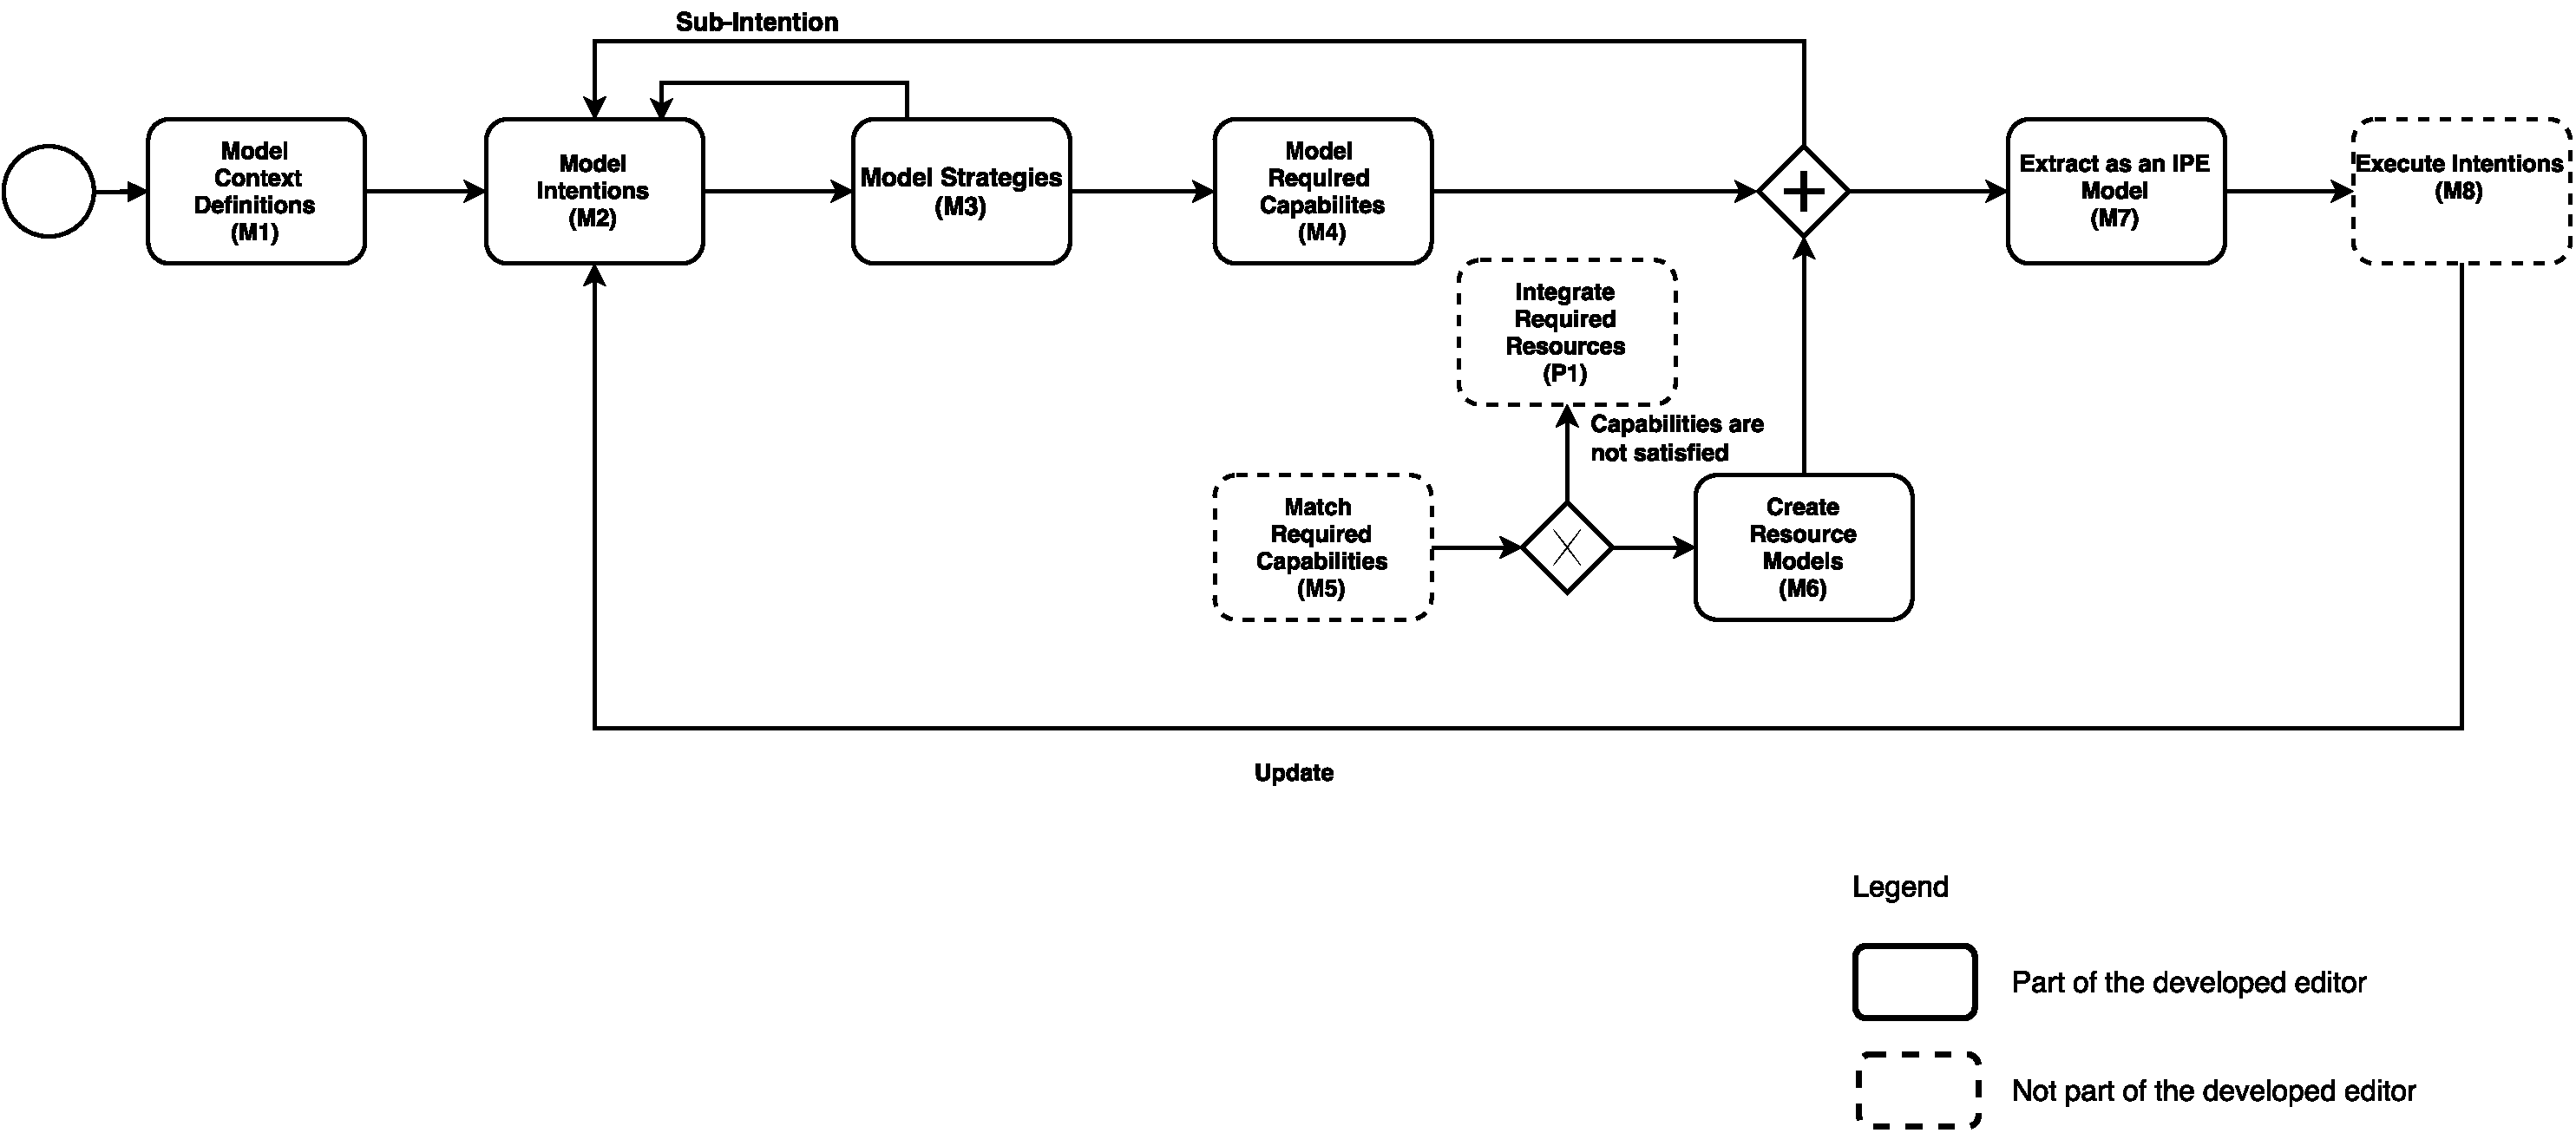
\includegraphics[width = \textwidth]{processmodeling.pdf}
	\caption{Steps of Model Informal Process}
	\label{fig:processdiagram}
\end{figure}

\subsubsection{Model Context Definitions (M1)}  
The first step is to model context definitions, where we can model both (1) basic properties like name and target namespace of a context definition and (2) entity specific properties like contained contexts, entity definitions, etc., of a context definition. For example, consider initial context from our motivating scenario in the Section \ref{sec:scenario}, we can provide meaningful name such as \textit{quarterly initial context}. We can also provide any valid target namespace URI of the context. Similarly, the user can also provide other entity specific properties of the context. 

\subsubsection{Model Intentions (M2)}  
Similar to context definition modeling (M1), the second step (M2) is to model intentions. The context definitions created in step M1 can be used to specify initial and final contexts of an intention. Intentions has any type of custom relationships among different intentions. For example, sub-intentions, contradicting intentions, etc. These type of sub intentions and contradicting intentions are also modeled as intentions in this step and their type of relation to a specific intention are mentioned. Intentions are associated with strategies. Strategies, required to achieve an intention are added to entity specific properties of intention as achieving strategies in this step. For example, in our motivating scenario the main intention \textit{increase revenue and number of unit sales} has three achieving strategies such as, (1) \textit{through expansion}, (2) \textit{through advertisements} and (3) \textit{through good customer support}. After providing basic properties of an intention such as name and target namespace, the user can provide entity specific properties such as details of achieving strategies, related intentions, etc.

\subsubsection{Model Strategies (M3)}  
Once intentions are identified and modeled, the third step (M3) is modeling of strategies, to achieve a specific intention. As mentioned earlier in the Section \ref{sec:entitytypesrepresentation}, an intention can have multiple strategies.  A strategy is a method or plan chosen to bring desired results, such as achievement of an intention or solution to a problem. Strategies are associated with capabilities. The capabilities required by strategy are added to entity specific properties of strategy in this step. For example, consider the strategy \textit{through expansion} from our motivating scenario. This step includes providing basic details of strategy such as name and target namespace. This step also includes providing entity specific properties of strategy such as target intention. For the strategy \textit{through expansion}, the target intention is main intention, i.e., \textit{increase revenue and number of unit sales}  

\subsubsection{Model Required Capabilities (M4)}  
After modeling of strategies, capabilities required to achieve an intention in a specific strategy are modeled. Strategies require capabilities to accomplish an intention. A capability describes the ability provided by a resource or required by an intention. The performers of an informal process should posses certain skills and roles to achieve the intention. These type of required skills are modeled during this step. For example, consider the intention \textit{expand geographically} in our motivating scenario, to accomplish this intention through the strategy \textit{through product sales distribution}, we require \textit{product sales distribution capability}. This capability can be provided by organizational resource \textit{sales agent}. Thus, in this step we model capabilities details such as (1) basic properties of a capability such as name and target namespace and (2) entity specific properties of a capability such as organizational resources providing the required capability, etc.

\subsubsection{Match Required Capabilities (M5)} 
After modeling required capabilities, the step (M5) is to match the organizational resources that provides required capability and the capability. In this step, we consider the capabilities of all the organizational resources are known and matching of the capabilities of organizational resources and the required capability are done during this step. Here, matching of the capabilities and capabilities is finding the correct organizational resource that has the capability to carry out the process. 

\subsubsection{Integrate Required Resources (P1)} 
If there is no suitable matching capability, then phase P1 of InProXec can be carried out again until a matching capability is found. In this phase of the InProXec method, technical experts develop services (1) to retrieve required information about the resources, (2) to acquire the resources and (3) to release the resources on process completion. Thus, this phase of InProXec helps in using the information available about resources during modeling \cite{Sungur2015}. If capabilities are satisfied, then the next step of creating resource models can be proceeded.

\subsubsection{Create Resource Models (M6)}  
After matching the resources and capabilities, the resource models are created. The need for modeling a new intention may arise in parallel during modeling of resources. As mentioned earlier, in our motivating scenario there can be a new requirement to support help desk through mobile. This results in requirement of a resource that provides \textit{mobile application developer capability}. A resource can be a people or tool that drive towards the successful execution of the process and it is a key for achieving specified process intentions. 

\subsubsection{Extract as an IPE Model (M7)}  
After the completion of above mentioned steps, the modeled strategy which is associated with a valid capability can be extracted as an IPE model. The IPE models realize the execution of a strategy in next step. 

\subsubsection{Achieve Intentions (M8)}
When all of the achieving strategies of an intention are successfully executed, i.e., IPE models realize the execution of strategy, it ends accomplishment of an intention. After achieving the intention, the intention is moved to its final context. For example, in our motivating scenario when the main intention \textit{increase revenue and number of unit sales} is accomplished then it reaches final context of \textit{increased revenue and sales for the quarter}. 

Another important information to mention here is, realizing the abstract concepts of steps (M5), (M6), (M7) and (M8) are not part of the current functioning system. This functioning system is developed to realize the proposed approach, this is explained in detail in the following Chapter \ref{chap:casestudy}  
 
%%%%%%%%%%%%%%%%%%%%%%%%%%%%%%%%%%%%%%%%%%%%%%%%%%%%%%%%%%%%%%%%%%%%%%%%%
\section{A Top-down Modeling Approach}
\label{sec:topdownapproach}
%%%%%%%%%%%%%%%%%%%%%%%%%%%%%%%%%%%%%%%%%%%%%%%%%%%%%%%%%%%%%%%%%%%%%%%%%
As we mentioned earlier, the modeling approach in our context is descriptive modeling approach which starts from top level intention and refines modeling until the operational bottom level is reached. Hence, it is called top-down modeling approach. The purpose of selecting top-down modeling approach is because based on the suggestions provided in the existing literatures \cite{Mandic2010, Bider2005,Sungur2016}. These literatures suggest that the value of an intention in the top of hierarchy propagates till the lower level and helps in making investment-related decisions while at the same time integrating cost and benefit estimates from all levels. Moreover, by creating declarative models, i.e., models that provide information in order to do accomplish an intention, using top-down modeling approach, models are easily changeable as they are decoupled from their operational terms, i.e., business process models. The integration of declarative models using top-down modeling approach, also provides coupling of the cost-benefit and strategy achievability estimation with operationally measurable business intention and supports the evaluation of business intention's success and the effectiveness of the chosen strategies. 

In the Figure \ref{fig:topdownapproach}, it is shown how this modeling approach starts modeling from top level intentions and does modeling until the operational lower level is reached and how the organizational modeling elements are associated with each other. In this approach, intentions at different levels can be viewed by organizational members. Also, in this approach the intentions are associated with the informal processes through the strategies. This makes the approach oriented to intention, when the participating process is associated with an intention. To successfully accomplish an organizational intention through this approach, members require understanding of the the intentions and its associated elements. This approach also enables modeling of intentions based on the input from different members from different groups of the organization. From the Figure \ref{fig:topdownapproach}, we could see that the required capabilities are provided by the organizational resources. When there exist organizational resources that can provide a capability, then the capability is called as \textit{valid capability}. In this approach, it is considered that cost of organizational resources are known and cost of executing a strategy can be estimated based on its association with resources through the required capabilities. 


\begin{figure}
	\centering
	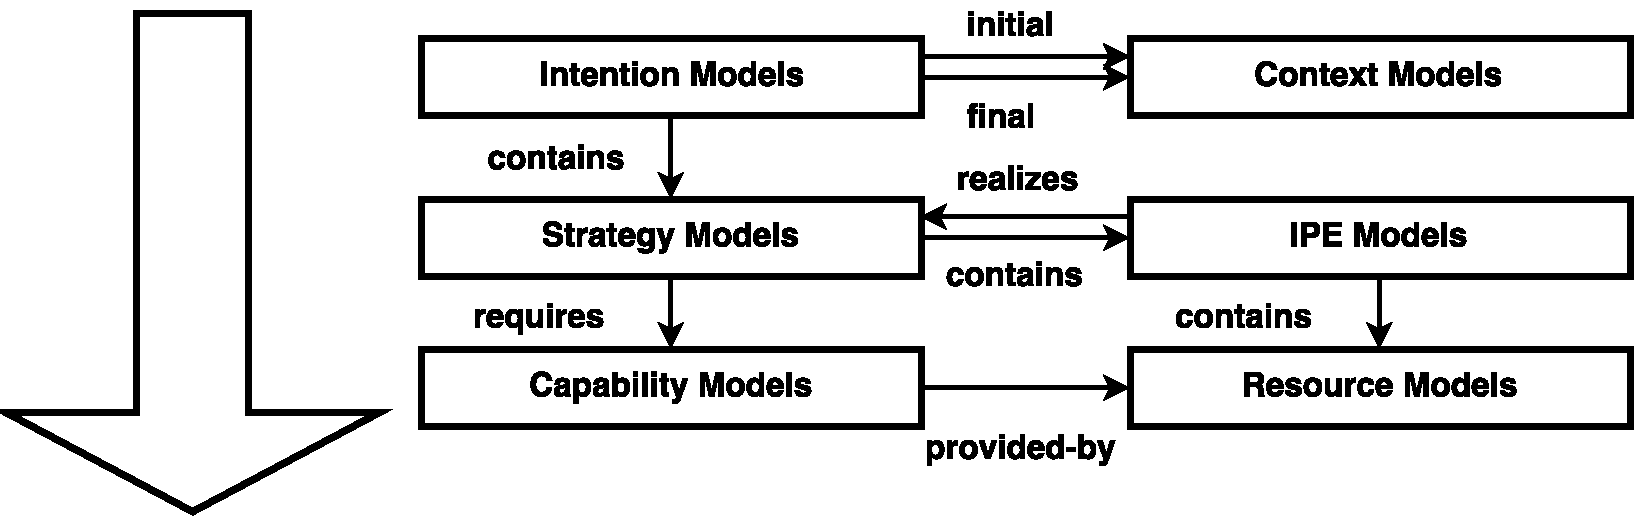
\includegraphics[width=\textwidth]{TopDownApproach.pdf}
	\caption{Intention-oriented Organizational Modeling - A Top down Modeling Approach}
	\label{fig:topdownapproach}
\end{figure}

The approach is evaluated based on the derived requirements in the Section \ref{sec:requirementssupoorting} of Chapter \ref{chap:analysis} as follows :

\textit{Organizational Intention Transparency} (R1) : From the Figure \ref{fig:topdownapproach}, one could understand that (1) intentions are refinable and as per the current design of the approach and (2) organizational members can view the intentions at different levels. Thus, requirement R1 is satisfied by the approach as it satisfies all of the pre-requisites. 

\textit{Organizational Strategy-based Cost Estimation} (R2) :  In this approach, (1) resources are associated with cost and (2) the cost estimation of strategies include its association with low level structures. Thus, requirement R2 is satisfied by the approach as it satisfies all of the pre-requisites. 

\textit{Organizational Strategy Achieve-ability Estimation} (R3) :  In this approach (1) a capability is considered as valid when there exist matching organizational resources and (2) from the Figure \ref{fig:topdownapproach}, one could understand how independent informal process realizes strategy. Thus, requirement R3 is satisfied by the approach as it satisfies all of the pre-requisites.

\textit{Intention Oriented Working Style} (R4) : This approach (1) satisfies requirement R1 and (2) this approach requires understanding of intention and its associated elements for successfully achieving the main intention. Thus, requirement R4 is satisfied by the approach as it satisfies all of the pre-requisites.

\textit{Participative Organizational Modeling} (R5) : This approach (1) satisfies requirement R1 and  (2) also enables intention modeling based on the input received from the organizational members. Thus, requirement R5 is satisfied by the approach as it satisfies all of the pre-requisites. 



